\subsection{ZooKeeper [SP]}

Large distributed systems require a coordinator for system configuration management.
As it was mentioned in Chapter 4, Google uses a Chubby service for this purpose.
The main Chubby disadvantage is that for lock and unlock operations it is necessary to open and close the object consequently.
This feature influences the performance, increasing the time needed for making a lock.
Therefore Yahoo develops its own service named ZooKeeper that manages systems configuration and allows to efficiently lock the shared resources.

ZooKeeper namespace looks similar to a standard file system \cite{Zookeeper}.
It consists of interconnected nodes, each of them identified by a path.
The path contains elements separated by a slash ('/').
Like in a file system, every node except the root has a parent node.
The parent node's path is a prefix for the current node path.
The ZooKeeper namespace differs from a standard file system in that its node can be a file and a directory simultaneously.

There are two types of nodes: persistent and ephemeral.
ZooKeeper stores persistent nodes on the disk, while ephemeral nodes belong to a particular session and exist only during this session.
Ephemeral nodes cannot have children nodes, they can only store data.
ZooKeeper client establishes a session with a ZooKeeper server, passing heartbeat messages.
When a client stops to receive heartbeat messages, it reconnects to a different server, reestablishing the session.
If the session is canceled, all its ephemeral nodes are automatically removed.
ZooKeeper tree is presented in Figure~\ref{fig:zookeeper_tree} where the dark nodes are ephemeral.

\begin{figure}
  \centering
  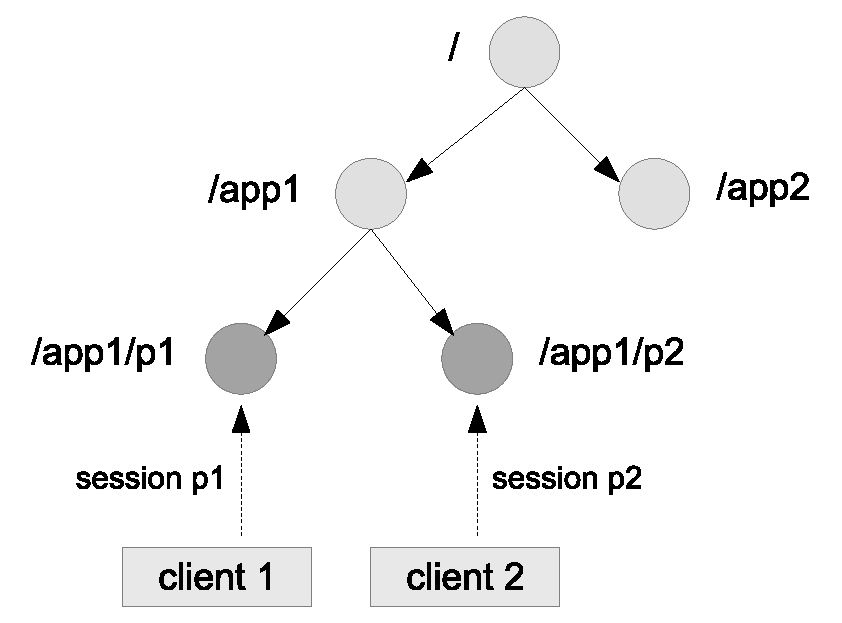
\includegraphics [width=0.5\textwidth]{images/zookeeper_tree}
  \caption{ZooKeeper tree sructure}
  \label{fig:zookeeper_tree}
\end{figure}

ZooKeeper is designed for small data warehousing, such as configuration, status and location information.
One node is usually not bigger than one kilobyte.
Therefore it stores data tree image in memory, keeping in a persistent store only transaction logs and snapshots.
In-memory storage limits the size of the database of ZooKeeper.
However, it gives advantages of low latency and high performance. 

The key feature of ZooKeeper is that it uses First In, First Out (FIFO) method for processing the messages.
It means that all commands are performed in the order they are received.
Thus, ZooKeeper maintains the total ordering.
The order is specified by a unique ZooKeeper Transaction id, that is assigned to each update.
 
ZooKeeper supports idempotent operations.
If a node should be updated, the system makes a note about the update and keeps an old and a new version of this node.
This allows client to receive the same message several times, being aware of when it can be applied.
Therefore all the write operations are performed sequentially in one thread and only on the master node.
On the contrary, read requests do not necessarily need the master node, they can be handled by a node's replica.

The client also supports the total ordering of the messages.
Hence if the client sends a write request and then a read request, the write operation is performed first.
Even if usually read operation does not need a lock, ZooKeeper strictly follows the order.
It allows to implement predictable asynchronous systems that work with ZooKeeper.

A client can watch a node.
If it sets a watch, it gets notified when the node is changed.
When the node sends this notification, it removes the watch.
In the case of connection problems between the client and the ZooKeeper server, the client receives a local notification.

ZooKeeper guarantees reliability using replication.
Its database is replicated to several nodes, one of them is a \textit{Leader} and the others are \textit{Followers}.
\textit{ZooKeeper Atomic Broadcast} (Zab) algorithm is used for managing the communication between the leader and the followers \cite{Medeiros2012}.
It synchronizes the replicas, broadcasts updates and recovers the valid state in the case of nodes crash.

Zab includes four phases: (1) Leader election, (2) Discovery, (3) Synchronization and (4) Broadcast.

1. On the first stage ZooKeeper uses any election algorithm to choose a leader.
After termination every node stores its vote locally in volatile memory.
When a node \textit{n} votes for a node \textit{n'}, \textit{n'} becomes a \textit{prospective leader} for \textit{n}.

2. On the second stage the nodes inform the prospective leader about the most recent transactions they accepted.
Thus the prospective leader knows the latest sequence af accepted transactions and can establish a new epoch.
From this moment the previous leaders cannot perform any commits.
In the case of connection problems between a follower and a leader, the follower goes back to the stage (1) of this algorithm.

3. The leader is aware of the latest transactions history and during this stage synchronizes this information with its replicas.
This phase is also called voting phase, because it receives the votes from the nodes.
The leader performs a commit only if it receives acknowledgements from two of three followers.
At this moment the leader changes its state from \textit{prospective} to \textit{established}.

4. The nodes persist in this stage until a crash.
Every write request from a ZooKeeper client is broadcasted among the nodes.
New followers can join, receiving the transaction history from the leader.
The leader and its followers use periodic heartbeat messages for early failure detection.
If any of the nodes do not receive a heartbeat message within a timeout, it shifts its state to \textit{election} and goes back to the first stage.

It can happen that one of the followers still has outdated information when it receives the read request.
To avoid this problem, it is possible to make a force synchronization with the master.
It is called the \textit{slow read}.
Evidently, if all the clients use the slow read the system loses the advantage of scaling.
Without force synchronization ZooKeeper system scales for reads nicely. 
However, in this case the client that reads from a replica can obtain the outdated information.